% !TEX root = ../../main.tex
\section{Hierarchical Clustering}\label{sec:rw_hc}

%%%%%%%%%%%%%%%%%%%%%
%dendrogram
%%%%%%%%%%%%%%%%%%%%%%
\begin{figure}[H]
    \centering
    \subfloat[Bottom-Up: Nodes are merged with increasing time]{\label{fig:hc_bottom_up}
        {
            \begin{tikzpicture}[sloped]
                \node (a)    at (-6,0)      {a};
                \node (b)    at (-5,0)      {b};
                \node (c)    at (-4,0)    {c};
                \node (d)    at (-3,0)     {d};
                \node (e)    at (-2,0)       {e};

                \node (ab)   at (-5.5,1)    {};
                \node (cd)   at (-3.5,1)    {};
                \node (cde)  at (-2.75,2)       {};
                \node (all)  at (-4,3)    {};
                
                \node (root) at (-4,4) {root}; 

                \draw (a) |- (ab.center);
                \draw (b) |- (ab.center);
                \draw (c) |- (cd.center);
                \draw (d) |- (cd.center);
                \draw (e) |- (cde.center);
                \draw (cd.center) |- (cde.center);
                \draw (ab.center) |- (all.center);
                \draw (cde.center) |- (all.center);
                \draw (all.center) |- (root.center);

                \draw[->,-triangle 60] (-7,0) -- node[above]{time} (-7,4);
            \end{tikzpicture}
        }
    }\hspace{2cm}
    \subfloat[Top-Down: Nodes are divided with increasing time]{\label{fig:hc_top_down}
        {
            \begin{tikzpicture}[sloped]
                \node (a)    at (-6,0)      {a};
                \node (b)    at (-5,0)      {b};
                \node (c)    at (-4,0)    {c};
                \node (d)    at (-3,0)     {d};
                \node (e)    at (-2,0)       {e};

                \node (ab)   at (-5.5,1)    {};
                \node (de)   at (-2.5,1)    {};
                \node (cde)  at (-3.25,2)       {};
                \node (all)  at (-4,3)    {};
                
                \node (root) at (-4,4) {root}; 

                \draw (a) |- (ab.center);
                \draw (b) |- (ab.center);
                \draw (c) |- (cde.center);
                \draw (d) |- (de.center);
                \draw (e) |- (de.center);        
                \draw (de.center) |- (cde.center);
                \draw (ab.center) |- (all.center);
                \draw (cde.center) |- (all.center);
                \draw (all.center) |- (root.center);

                \draw [->,-triangle 60] (-7,4) -- node[below,align=center]{time} (-7,0);
            \end{tikzpicture}
        }
    }
    \addtocontents{lof}{%
    \vspace{1cm}
    \protect\centerline{%
    \protect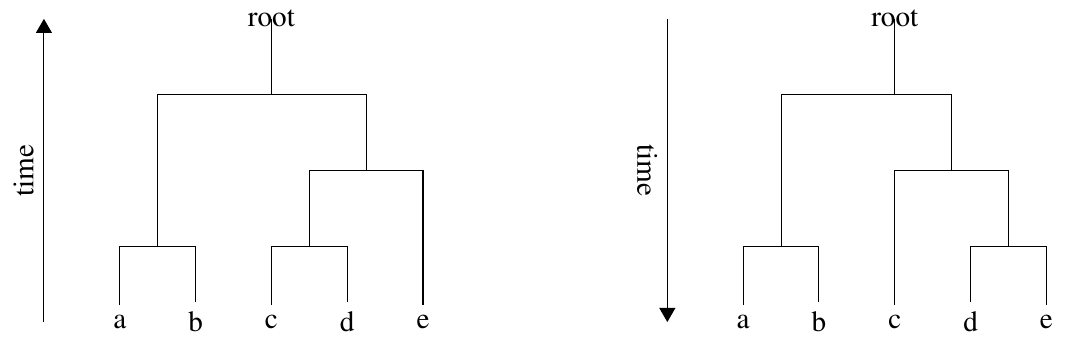
\includegraphics[width=.2\linewidth]{fig/thump/dendro.png}
    }%
    }%
    \caption[Bottom-up vs. top-down hierarchical clustering]{
        Bottom-Up clustering: Nodes are merged with increasing time.
        At the begin, all nodes are leafs, and they are merged
        together.
        Top-Down clustering: Nodes are divided with increasing time.
        At the begin, all nodes are in the root of the tree,
        and with increasing time, nodes are split.

    }
    \label{fig:hc_bottom_up_top_down}
\end{figure}


Hierarchical clustering techniques have been successfully used
in computer vision since decades \citep{ohlander_1978_cgip,forsyth_2002_book,arbelaez_2006_cvpr,iglesias_2013,morel_1995_book}.

The method  of \citet{ohlander_1978_cgip} is an example for \emph{top-down} clustering,
where all pixels start in one single cluster. Each cluster is recursively divided 
into  more clusters. The method proposed in \cref{ch:cgc} has a strong connection to
\emph{top-down} clustering.
\citet{arbelaez_2006_cvpr} and \citet{iglesias_2013} use the bottom-up approach,
also called \emph{agglomerative clustering}, where 
adjacent nodes in a graph are merged iteratively to create 
a set of nested segmentations.


Such a hierarchy of clusters can be visualized as a dendrogram (see \cref{fig:hc_bottom_up_top_down} ).
The dendrogram can be interpreted as a tree where each node represents a
region in the image.
The leafs in the tree are the atomic units of the image (e.g. pixels, super-pixels or super-voxels)
and the root note is the entire scene itself (e.g. the complete image / graph).

There are a few differences between classic unstructured agglomerative clustering
\citep{florek_1951,sokal_1958_science_bulletin,ward_63_jasa}
and agglomerative clustering on graph data structures \citep{arbelaez_2006_cvpr,iglesias_2013,morel_1995_book}, 
e.g. grid-graphs and region adjacency graphs\citep{vlachos_1993_csv}.
While in unstructured hierarchical clustering, any pair of observations can be merged,
for graph hierarchical clustering, only adjacent nodes / regions can be merged.
In the literature this is also called ``hierarchical clustering with connectivity constraints'' \cite{scikit_learn}.


The main idea behind agglomerative clustering is very simple:

Initially, all observations start in a single cluster. 
Next, clusters which have highest similarities will be merged
iteratively.
Due to this merging, similarities change and need to be updated
/ recomputed. Therefore  noisy initial features
 become more informative.


\begin{table}
\begin{scriptsize}
\begin{tabular}{ |l|l|p{5cm}|}
    \hline 
    Euclidean Distance
        & $||a-b||_2 = \sqrt{\sum{ (a_i-b_i })^2 } $
        & For low dimensional data \\  \hline 
    Squared Euclidean Distance
        & $||a-b||_2^2 = \sum{ (a_i-b_i })^2  $
        & For low dimensions data\\  \hline
    Manhattan Distance
        &  $||a-b||_1 = \sum{ |a_i-b_i |}  $
        & Multi purpose \\  \hline 
    $\mathcal{X}^2$-Distance  
        &  $\frac{1}{2}\sum{  \frac{(a_i-b_i)^2}{a_i+b_i} }$
        & For histograms \\  \hline 
    Earth Mover  Distance          
        &  see \citet{levina_2001_iccv} 
        & For histograms \\  \hline 

\end{tabular}

\end{scriptsize}
\caption{
    An overview of the most common distances measurements and their main properties.
}\label{tab:hc_distance_types}
\end{table}



\begin{table}
\begin{scriptsize}
\begin{tabular}{ |l|l|p{5cm}|}
    \hline
    Average Linkage \citep{sokal_1958_science_bulletin}           
        & $d_{al}(C_a,C_b) = \frac{1}{|C_a||C_b|} \sum _{a \in C_a} \sum_{b \in C_b} d(a,b) $ 
        & \scriptsize Prefers clusters with same variance \cite{sokal_1958_science_bulletin} \\ \hline

    Single Linkage \citep{florek_1951}            
        & $d_{sl}(C_a,C_b) =  \min\{d(a,b) : a \in C_a, b \in C_b\}$ 
        & Nice theoretic properties \citep{hartigan_1981_jjamstat,milligan_1980_psycho}, can lead
          to very irregular shaped clusters \\ \hline
    Complete Linkage \citep{sorensen_1948}         
        & $d_{cl}(C_a,C_b) =  \max\{d(a,b) : a \in C_a, b \in C_b\}$ 
        & Prefers clusters with same diameter \citep{milligan_1980_psycho} \\ \hline
    Centroid Distance         
        & $d_{cd}(C_a,C_b) =  d(\bar{C}_a,\bar{C}_b) $ 
        & Robust w.r.t. outliers \citep{milligan_1980_psycho} \\ \hline
    Wards Minimum Variance \citep{ward_63_jasa}
        & $d_{wmv}(C_a,C_b) = \frac{ d(\bar{C}_a,\bar{C}_b)}{ \frac{1}{|C_a|} + \frac{1}{|C_b|} } $ 
        & Prefers clusters with same size, is sensible to outliers \citep{milligan_1980_psycho} \\ \hline
\end{tabular}

\end{scriptsize}

\caption{
    The distance between to clusters is usually based on the 
    individual distance between elements within the clusters.
    These distance are \emph{linked} together.
    An overview of the most common cluster distances linkages and their main properties.
}\label{tab:hc_linkage_types}
\end{table}


The definition of a specific distance betweens clusters is crucial, 
but strongly depends on the application.
The distance between two clusters is usually based on the 
individual distance between elements within the clusters.
These distance are then \emph{linked} together using a specific linkage type.
\Cref{tab:hc_distance_types} gives a short overview of many common distance
types and \cref{tab:hc_linkage_types} gives a  brief overview 
of most common cluster linkage types and their main properties.








\iffalse
\begin{tikzpicture}[scale=  1,every node/.style={minimum size=1cm},on grid]
        
    %slanting: production of a set of n 'laminae' to be piled up. N=number of grids.
    

    %%%%%%%%%%%%%%%%%%%%%%%%%%%%%%%%%%%%%%%%%%%%%%%%%%%%%%%%%%%%%%%
    % 0 bottom layer
    %%%%%%%%%%%%%%%%%%%%%%%%%%%%%%%%%%%%%%%%%%%%%%%%%%%%%%%%%%%%%%%%
        
    \begin{scope}[yshift=0,every node/.append style={yslant=0.5,xslant=-1},yslant=0.5,xslant=-1]
        \draw[-latex,thick] (-0.17,3.21/2) node[right]{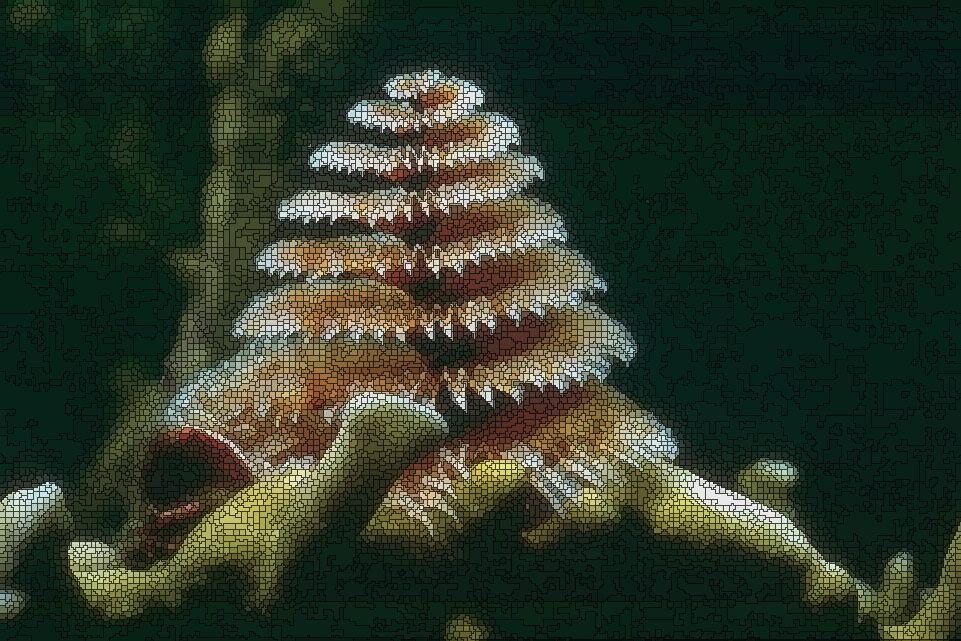
\includegraphics[width=4.82cm]{fig/12074/0.png}};
        \draw[black,very thick] (0,0) rectangle (4.81,3.21);
    \end{scope}

    \begin{scope}[yshift=60*1,every node/.append style={yslant=0.5,xslant=-1},yslant=0.5,xslant=-1]
        \draw[-latex,thick] (-0.17,3.21/2) node[right]{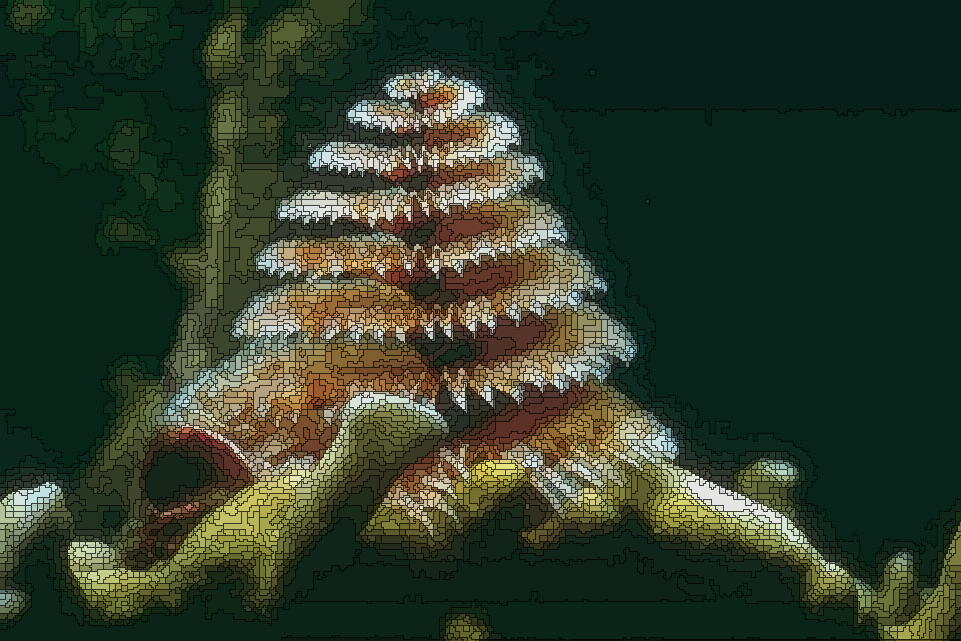
\includegraphics[width=4.82cm]{fig/12074/2.png}};
        \draw[black,very thick] (0,0) rectangle (4.81,3.21);
    \end{scope}

    \begin{scope}[yshift=60*2,every node/.append style={yslant=0.5,xslant=-1},yslant=0.5,xslant=-1]
        \draw[-latex,thick] (-0.17,3.21/2) node[right]{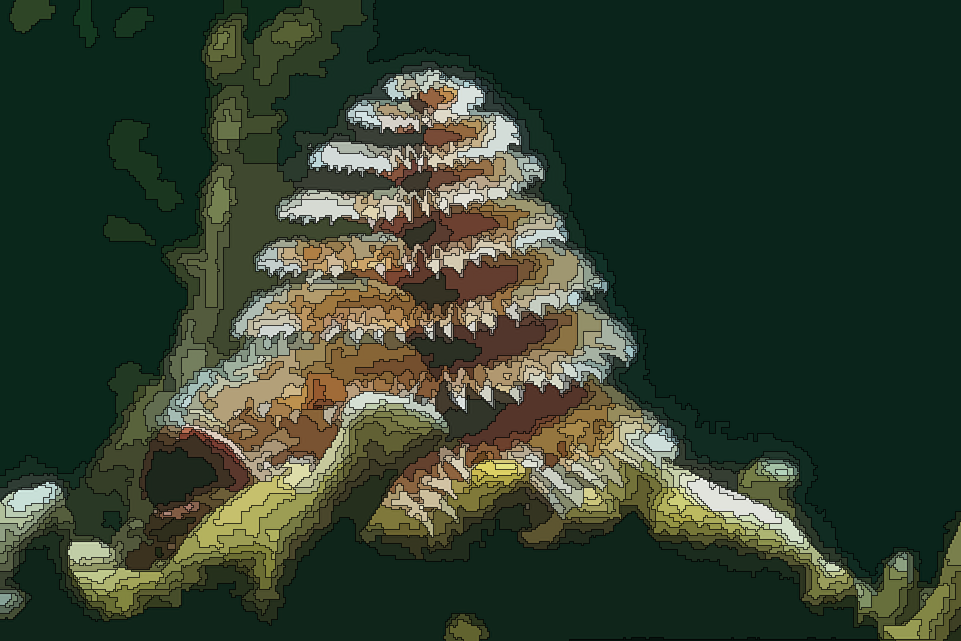
\includegraphics[width=4.82cm]{fig/12074/4.png}};
        \draw[black,very thick] (0,0) rectangle (4.81,3.21);
    \end{scope}

    \begin{scope}[yshift=60*3,every node/.append style={yslant=0.5,xslant=-1},yslant=0.5,xslant=-1]
        \draw[-latex,thick] (-0.17,3.21/2) node[right]{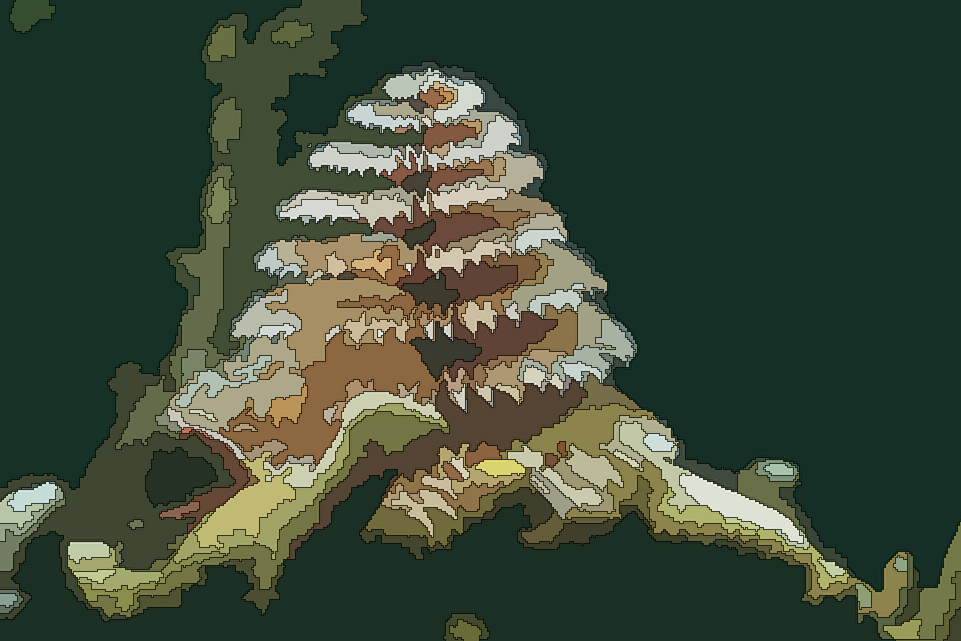
\includegraphics[width=4.82cm]{fig/12074/6.png}};
        \draw[black,very thick] (0,0) rectangle (4.81,3.21);
    \end{scope}

    \begin{scope}[yshift=60*4,every node/.append style={yslant=0.5,xslant=-1},yslant=0.5,xslant=-1]
        \draw[-latex,thick] (-0.17,3.21/2) node[right]{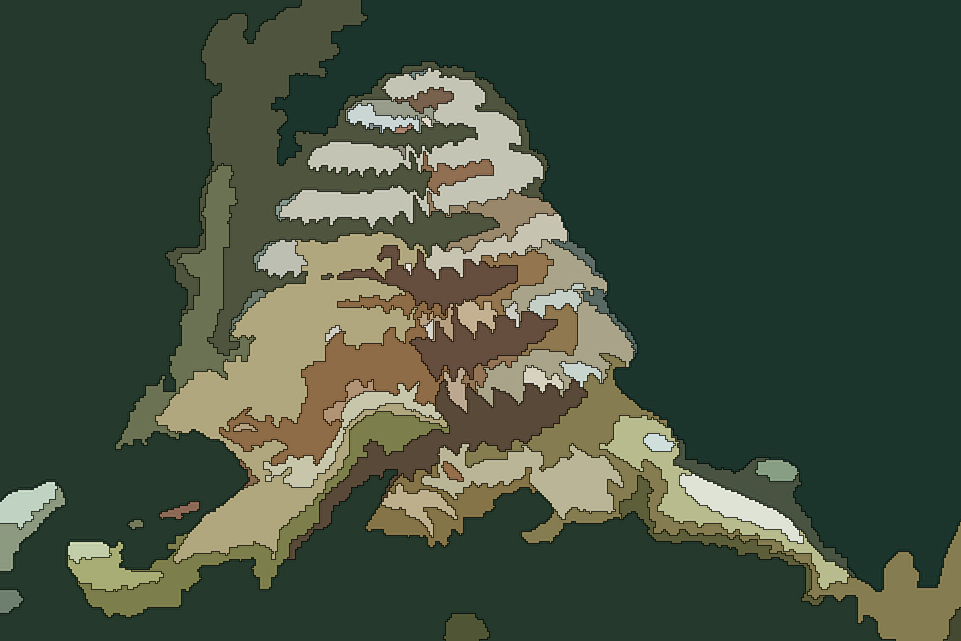
\includegraphics[width=4.82cm]{fig/12074/8.png}};
        \draw[black,very thick] (0,0) rectangle (4.81,3.21);
    \end{scope}


    \draw[->,-triangle 60] (-3,0) -- node[above]{time} (-3,4);

    %%%%%%%%%%%%%%%%%%%%%%%%%%%%%%%%%%%%%%%%%%%%%%%%%%%%%%%%%%%%%%%
    % 0 bottom layer
    %%%%%%%%%%%%%%%%%%%%%%%%%%%%%%%%%%%%%%%%%%%%%%%%%%%%%%%%%%%%%%%%
    \draw[-latex,thick] (6.2,2) node[right]{$\mathsf{over-segmentation}$}
         to[out=180,in=90] (4,2);
         
         
         
    %%%%%%%%%%%%%%%%%%%%%%%%%%%%%%%%%%%%%%%%%%%%%%%%%%%%%%%%%%%%%%%
    % 1 layer
    %%%%%%%%%%%%%%%%%%%%%%%%%%%%%%%%%%%%%%%%%%%%%%%%%%%%%%%%%%%%%%%%
    
    \draw[-latex,thick] (6.2,5.5) node[right]{$\mathsf{Region adjacency graph 1}$}
         to[out=180,in=90] (4,5.5);
\end{tikzpicture}
\fi







In the case of graph hierarchical clustering, informative features
can also be attached to the edges of the graph.
Edge detectors such as the gradient magnitude, gPb \citep{marie_2008_cvpr}  or learned
edge detectors \cite{dollar_2013_iccv}  can be used to boost performance
of agglomerative clustering \citep{arbelaez_2006_cvpr,iglesias_2013}.


\citet{ arbelaez_2006_cvpr} introduce the following notation:
They use $\Omega \in \mathbb{R}^2$ as image domain.
$P_0$ is the initial partition and they define a
\emph{hierarchical segmentation operator} (HSO) which
assigns a partition $P_\lambda$ given the initial partition and
a scale parameter $\lambda$.
Furthermore the following properties must be fulfilled for a HSO:  

\begin{align} 
P_{\lambda}  =  P_0 ,\hspace{0.5cm}  \forall \lambda \leq 0  \label{eq:ucm_hco_eq_0} \\ 
\exists \lambda_1 \in \mathbb{R}^+  : P_{\lambda}  =  \{ \Omega \} ,\hspace{0.5cm} \forall \lambda \geq \lambda_1  \label{eq:ucm_hco_eq_1} \\
\lambda < \lambda'  \rightarrow  P_{\lambda} \sqsubseteq   P_{\lambda'} \label{eq:ucm_hco_eq_2}
\end{align}


\Cref{eq:ucm_hco_eq_0} and \cref{eq:ucm_hco_eq_1}  give $\lambda$ a range.
\Cref{eq:ucm_hco_eq_2} ensures that the segmentations are nested.
They define the \emph{saliency} of a contour as the scale $\lambda$ where
the contour disappears (see \cref{fig:ucm_visu}).
Thresholding the saliency map leads to closed contours.
As a consequence, the complete hierarchical segmentation
generated by a HSO can be encoded in the saliency map (see \cref{fig:ucm_saliency}).


\citet{iglesias_2013} improve segmentation results by combining 
agglomerative clustering combined machine learning.
Their main idea is to combine training data at multiple scales
which are generated during the region merging process.
This approach outperforms single scale learning.


\begin{figure} 
    \begin{center}
        \subfloat[$K_0$]{ \label{fig:ucm_k0}
            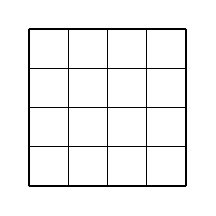
\begin{tikzpicture}
                \draw[step=0.5,black,thin] (0.0,0.0) grid (2,2);
                \draw[step=2,black,thick] (0.0,0.0) grid (2,2);
            \end{tikzpicture}
        }
        \hspace{0.5cm}
        %
        %
        %
        \subfloat[$K_1$]{ \label{fig:ucm_k1}
            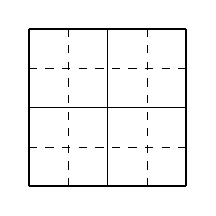
\begin{tikzpicture}
                \draw[step=0.5,black,very thin,dashed] (0.0,0.0) grid (2,2);
                \draw[step=1,black,thin] (0.0,0.0) grid (2,2);
                \draw[step=2,black,thick] (0.0,0.0) grid (2,2);
            \end{tikzpicture}
        }
        \hspace{0.5cm} 
        %
        %
        %
        \subfloat[$K_2$]{\label{fig:ucm_k2}
            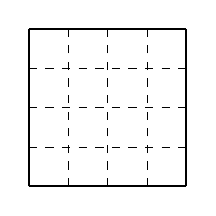
\begin{tikzpicture}
                \draw[step=0.5,black,very thin,dashed] (0.0,0.0) grid (2,2);
                \draw[step=2,black,thick] (0.0,0.0) grid (2,2);
            \end{tikzpicture}
        }
        \hspace{0.5cm}
        %
        %
        %
        \subfloat[$\mathcal{C}(\Upsilon) $]{ \label{fig:ucm_saliency}
            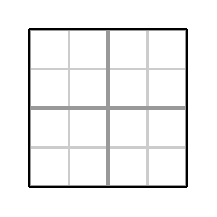
\begin{tikzpicture}
                \draw[step=0.5,black!20,thick] (0.0,0.0) grid (2,2);
                \draw[step=1,  black!40,very thick] (0.0,0.0) grid (2,2);
                 \draw[step=2,black,thick] (0.0,0.0) grid (2,2);
            \end{tikzpicture}
        }
        \hspace{0.5cm}
        %
        %
        %
        \subfloat[$\mathcal{C}(\Upsilon) $]{ \label{fig:ucm_saliency_3d}
            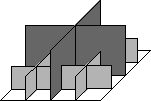
\includegraphics[width=0.2\textwidth]{fig/ucm3d.pdf}
        }
    \end{center}
    \addtocontents{lof}{%
    \vspace{1cm}
    \protect\centerline{%
        \protect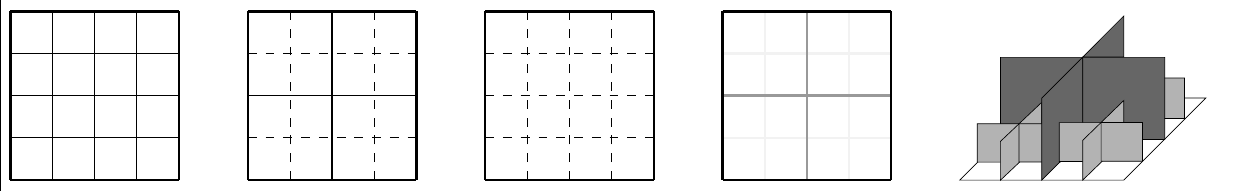
\includegraphics[width=.2\linewidth]{fig/thump/ucm.png} 
    }%
    }%
    \caption[Ultra metric contour map saliency]{
        \Cref{fig:ucm_k0} shows the a $4x4$ grid graph which serves as initial segmentation $K_0$.
        \Cref{fig:ucm_k1} shows the segmentation $K_1$ after the contraction of a few edges.
        Contracted edges are shown dashed.
        \Cref{fig:ucm_k2} shows the graph after all edges have been contracted.
        \Cref{fig:ucm_saliency} shows the saliency $\mathcal{C}$ of the contour $\Upsilon$.
        In \cref{fig:ucm_saliency_3d} the saliency from \ref{fig:ucm_saliency} is
        showed as a 3D visualization.
        This figure is very much inspired by \citep{arbelaez_2006_cvpr}.
    }\label{fig:ucm_visu}
\end{figure}




\Citet{najman_1994_sp} showed that there is a
strong connection between hierarchical segmentations
and watersheds.
They prove that there exists a bijection between
the set of ultrametric watersheds\citep{najman_2010_corr} and the set of hierarchical segmentations.
Furthermore, a recursive application of the watershed transformation  can
be used to generate a hierarchy of nested segmentations.
This transformation is called \emph{waterfall transformation} \citep{beuchner_1994_waterfall} .
